\section{First Member}
This is the section dedicated to one of the team members, and it should be written individually . It can include a range of things; first subsection is a space for you to point out the strengths and weaknesses of the module, including complaints about the module coordinator Max Wilson. The second section should have a selfie image with Max! The last part of it is the most important one. You will need to write a paragraph about what you have learned in this module. You can write it in \textbf{Bold} if you want or you can use other fonts. 

Please do not forget:
\begin{itemize}
	\item First paragraph should have your comments about the module
	\item Second one, a selfie img with Max
	\item Last one, what you learned in this module.
\end{itemize}

\subsection{Comments about the module}
The module has been interesting for showing proper methodologies for working on proper software projects, which are especially useful. The lectures have been well taught, and there is a wealth of additional information available on moodle which has been very helpful. The labs have been stressful at times, so probably the most taxing part of the module, but have at least been a good experience with the team and hasn't managed to destroy any friendships yet.

\subsection{Selfie with Max}

To include an image, you will need to remove the comments from the code below, place an image in the main folder, and do not forget to put the name of the image instead of ImgName. 

\begin{figure}[h]
\caption{Selfie with Max, photobombed by Liam}
\centering
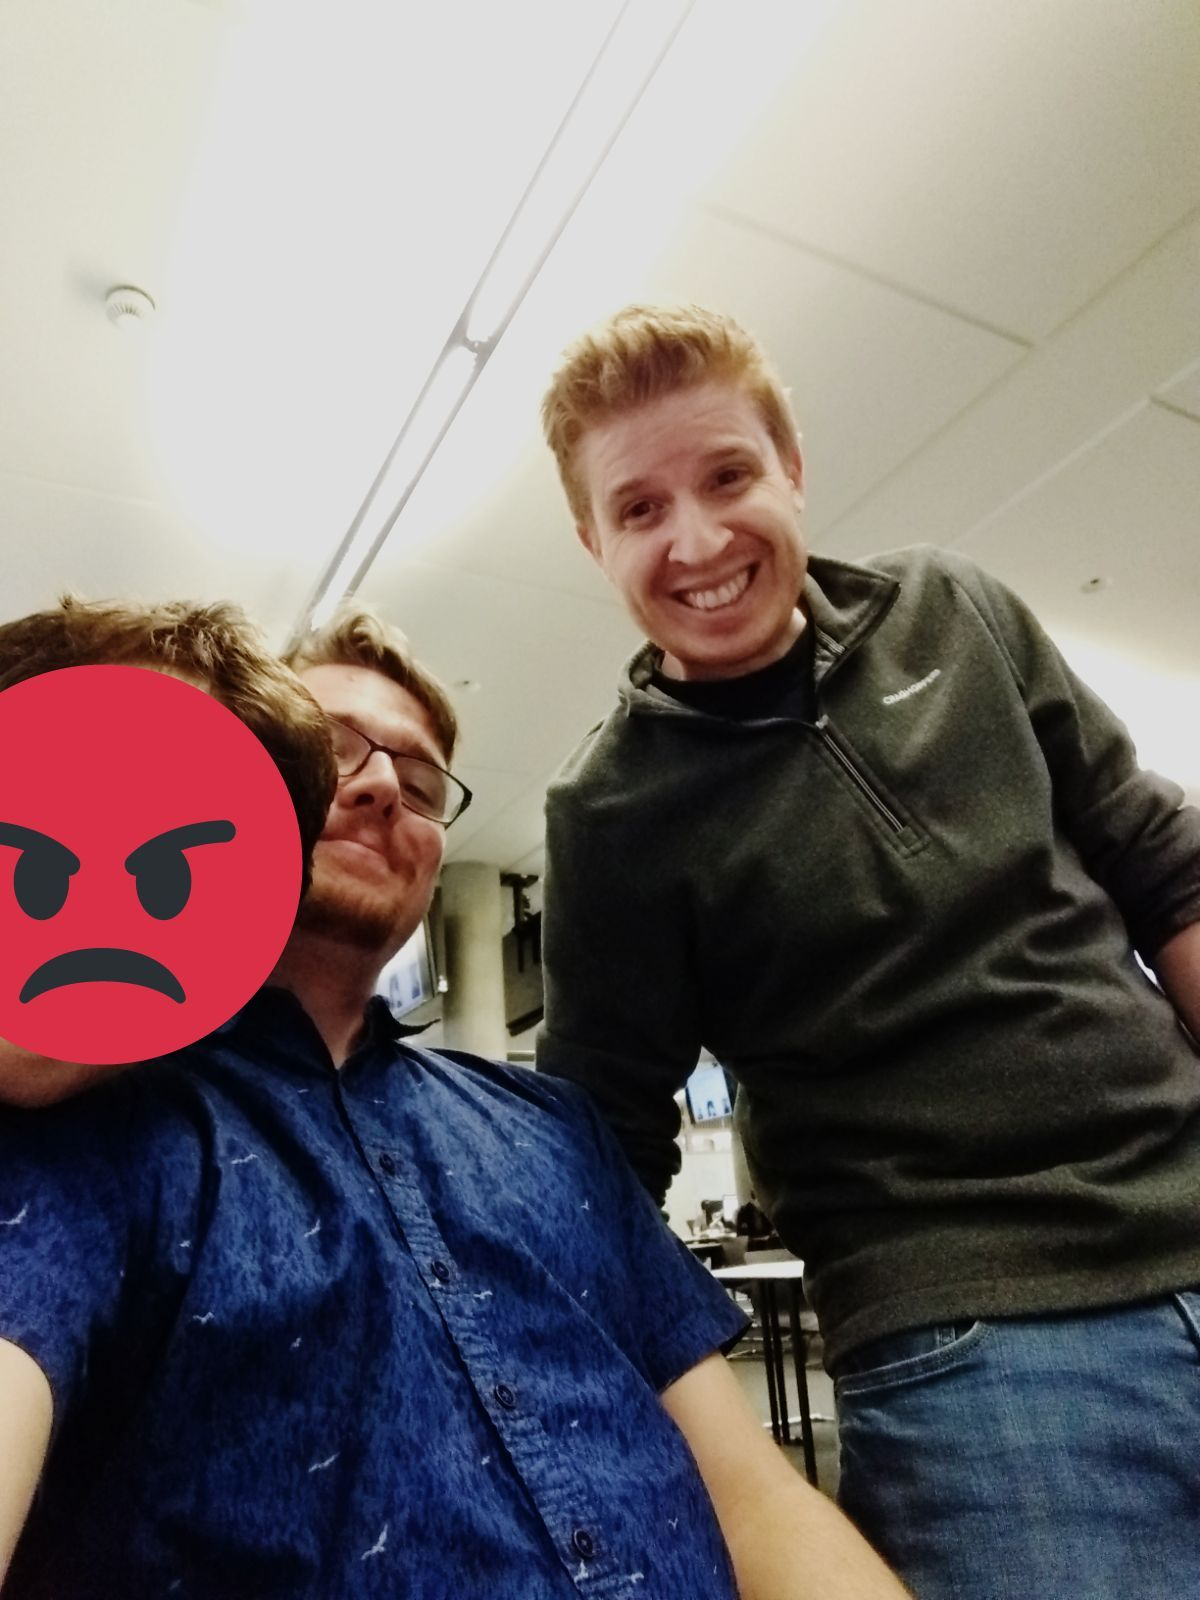
\includegraphics[width=0.5\textwidth]{MaxSelfie1.jpg}
\label{fig:selfie}
\end{figure}

You can then use the label of the figure to reference it later with the command ${\backslash}ref$. you can comment out the next line to see an example of how it works.

My selfie with Max is in  Figure~\ref{fig:selfie}.

\subsection{What I have learned in this module}
This module has taught me the value of really planning out work before beginning writing code, especially for large projects or when in teams. I have also learnt detail about specific models and techniques used in software development such the v-model as well as information about the various stages of software engineering. How to properly gather requirements, how to use these to inform specifications, how to plan testing, develop to specifications and then properly test through unit testing and acceptance testing to reach a finished project before continuing to maintain it after release. labs have also taught teamwork, as I have been mostly in charge of organising the groups, delegating work and making sure it is all done on time as well as doing my own share of the work and helping collate it to produce the final product. Working with the pressure of deadlines has been stressful, but overall a fulfilling experience.
